\chapter{Field Programmable Gate Array}

\section{Introduzione}
\begin{figure}[H]
    \centering
    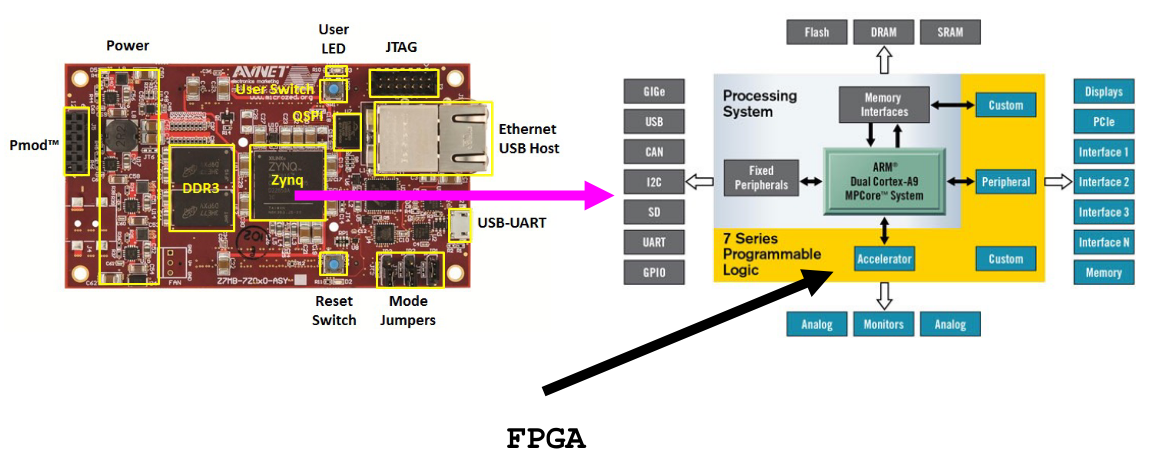
\includegraphics[width=0.6\textwidth]{/home/riccardoob/appunti/sistemi_digitali/images/6.png}
\end{figure}

Una FPGA è composta da \textbf{Configurable Logic Blocks} (CLB) che possono essere connessi con linguaggi ad alto livello (HDL o HDS).

Sono riprogrammabili sul campo e hanno un costo molto contenuto, sono supportate inoltre da linguaggio di alto livello come C, C++ o Python.

Sono la soluzione ideale per lo sviluppo veloce di prototipi e introdurli sul mercato in poco tempo. Un'altro grande vantaggio delle FPGA consiste nel fatto che hanno un consumo energetico molto basso. 

Permettono in generale un alto livello di astrazione, consentendo l'implementazione di reti logiche e algoritmi a livello hardware.

\section{Architettura FPGA}
Una FPGA è composta da migliaia di CLB, le funzioni e connessioni di ognuno di questi possono essere completamente progettate e riadattate sul campo dallo sviluppatore, che può generare nuove architetture molteplici volte.

Altre caratteristiche:
\begin{itemize}
    \item spesso le FPGA contengono anche RAM integrata (qualche KB)
    \item alcuni CLB sono dedicate alla gestione dell'I/O
    \item numerosi adder, multiplier etc.
\end{itemize}

\newpage
FPGA prodotte da diversi produttori si distinguono grazie a due aspetti:
\begin{itemize}
    \item Tecnologia usata per le connessioni
    \begin{itemize}
        \item fusibili
        \item memorie flash
        \item memorie SRAM
    \end{itemize}
    \item Struttura dei CLB
\end{itemize}

La figura sotto mostra la rete logica di una \textbf{Logic Cell} che implementa un CLB.
\begin{figure}[H]
    \centering
    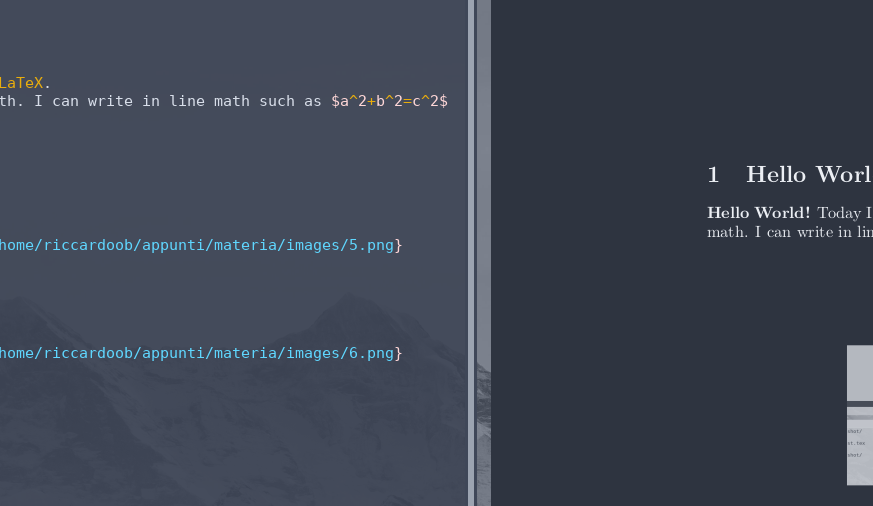
\includegraphics[width=0.7\textwidth]{/home/riccardoob/appunti/sistemi_digitali/images/7.png}
\end{figure}

Il blocco LUT è una rete combinatoria programmabile, può essere configurate per agire come uno shift-register o una memoria (RAM distribuita).

Tipicamente le Logic Cell sono raggruppate in \textbf{slice}, queste slice possono poi essere organizzate ulteriormente in gruppi per andare a formare un completo CLB.

\begin{figure}[H]
    \centering
    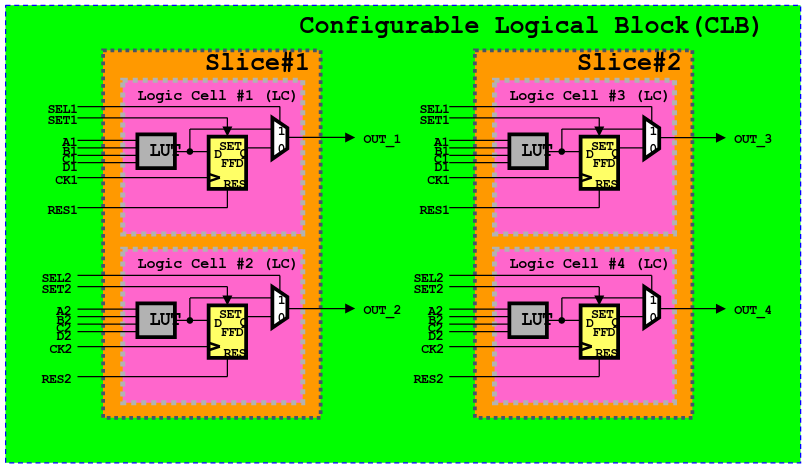
\includegraphics[width=0.7\textwidth]{/home/riccardoob/appunti/sistemi_digitali/images/8.png}
\end{figure}

La struttura effettiva di una FPGA, oltre ai CLB, comprende anche altre unità come la RAM e i multiplier:
\begin{figure}[H]
    \centering
    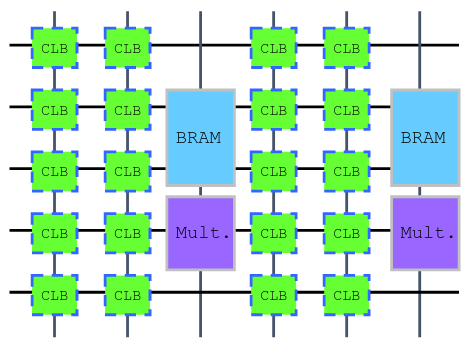
\includegraphics[width=0.5\textwidth]{/home/riccardoob/appunti/sistemi_digitali/images/9.png}
\end{figure}

\subsection{Clock}
Le FPGA sono solitamente configurate per implementare reti sincrone, quindi almeno un segnale di clock è necessario, usato per Sequential Synchronous Networks.

Spesso più domini di clock possono coesistere in uno stesso progetto, ad esempio ognuno dedicate a un particolare modulo, questo tuttavia crea problemi in caso sia necessario comunicare tra domini.
Per generare questi segnali clock a una frequenza prefissata, i produttori mettono a disposizione componenti specifici, chiamati \textbf{DCM} e \textbf{PLL}.
\\\\
Il clock è afflitto da due imprecisioni principali: lo \textbf{skew} e il \textbf{jitter}. Lo \textit{skew} produce uno sfasamento del del segnale mentre il \textit{jitter} causa una imprecisione dinamica nella frequenza del clock.

\begin{figure}[H]
    \caption{Skew e jitter}
    \centering
    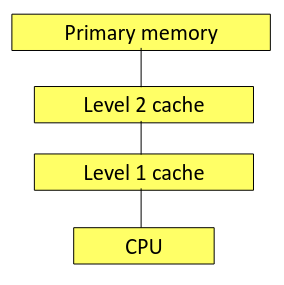
\includegraphics[width=0.6\textwidth]{/home/riccardoob/appunti/sistemi_digitali/images/10.png}
\end{figure}

Per ovviare a questi problemi si utilizzano i sopracitati DCM e PLL, aiutano a gestire il segnale del clock permettendo di:
\begin{itemize}
    \item generare segnali stabili, partendo da un segnale periodico esterno
    \item ridurre skew e jitter
    \item generare segnali con uno shift dato rispetto al segnale di reference
\end{itemize}

\subsection{IP-core}
Nelle FPGA è possibile utilizzare dispositivi comuni tramite gli \textbf{IP-core}, la controparte hardware delle librerie software).

Spesso questi IP-core sono basati su funzioni logice cablate nei circuiti dell'FPGA dai produttori (DCM e PLL sono alcuni di questi), alcuni esempi:
\begin{itemize}
    \item \underline{Memory controllers}, permettono di trasferire dati con dispositivi di memoria esterni
    \item \underline{Serializer/Deserializer} (SERDES), dispositivi per convertire segnali ad alta frequenza da seriale a parallelo (e viceversa)
    \item \underline{Communication controllers}, dispositivi per gestire trasferimenti ad alta larghezza di banda
\end{itemize}

Un IP-core configura una FPGA per implementare una specifica funzionalità, come per il software possono essere a pagamento, possono essere copiati tramite attacchi (SRAM) ma esistono comunque meccanismi di protezione.

\subsection{Frequenza e performance}
Le FPGA non hanno frequenze di clock alte, ottengono pero ottime performance grazie a 












































